\input{../include/preamble}

\title[ID1019 Parallel programming]{Parallel programming}
 

\author{Johan Montelius}
\institute{KTH}
\date{\semester}

\begin{document}

\begin{frame}
\titlepage
\end{frame}

\begin{frame}{Parallelism}

Parallelism vs Concurrency 

\vspace{20pt}

\begin{columns}
 \begin{column}{0.5\linewidth}
  Concurrency:
  \begin{itemize}
    \item multiple threads of control
    \item structure of architecture
    \item particularly suited for interactive applications
  \end{itemize}
 \end{column}
 \pause
 \begin{column}{0.5\linewidth}
  Parallelism:
   \begin{itemize}
    \item main goal - increase performance
    \item make use of parallel hardware
  \end{itemize}
 \end{column}
\end{columns}

\pause\vspace{10pt}{\em A concurrent program could be parallelized.}

\end{frame}

\begin{frame}{types of parallel hardware}

\begin{itemize}
  \pause\item Multiple Instructions Multiple Data (MIMD) : what is
  provided by a multi-core CPU but also by a distributed system

\pause\item Single Instruction Multiple Data (SIMD): typically used by
graphics cards, the same operations should be performed but on many
objects or pixels

\pause\item Pipeline : processing units that work in series, for
example the stages of execution of an instruction in a CPU

\end{itemize}

\pause\vspace{20pt}

{\em We will try to utilize a MIMD architecture.}

\end{frame}

\begin{frame}{types of parallel programming}

Several models of parallel computations:

\pause\vspace{20pt}

\begin{itemize}
 \pause\item loop parallelism: identify a loop where each iteration is independent
 \pause\item map-reduce: for each element in a set - perform an operation and collect the result
 \pause\item task parallelism: independent tasks are generated and executed in parallel
 \pause\item stream parallelism: a stream of events should be processes by several combinators
\end{itemize}

\pause\vspace{10pt}{\em A concurrent program could be executed in parallel but the focus is then concurrency not parallelism.}
\end{frame}

\begin{frame}{language support}

What language support do we have:

\begin{itemize}
 \pause\item parallel operators: extraction of parallelism by compiler, loop parallelism, map-reduce etc
 \pause\item concurrency:  concurrent processes that the can be execute in parallel
   \begin{itemize}
     \pause\item synchronization by shared memory/objects - Java, C++, ...
     \pause\item synchronization by message passing - Erlang/Elixir, Go, MPI, ...
   \end{itemize}
\end{itemize}

\end{frame}


\begin{frame}[fragile]{how do we exploit parallelism}

\begin{columns}
 \begin{column}{0.5\linewidth}
\begin{verbatim}
def fib(0) do 0 end
def fib(1) do 1 end
def fib(n) do
   f1 = fib(n-1),
   f2 = fib(n-2),
   f1 + f2
end
\end{verbatim}
 \end{column}
\pause
 \begin{column}{0.5\linewidth}
\begin{verbatim}
def fib(0) do 0 end
def fib(1) do 1 end
def fib(n) do
   f1 = spawn(fn() -> fib(n-1) end)
   f2 = spawn(fn() -> fib(n-2) end)
   f1 + f2
end
\end{verbatim}
 \end{column}
\end{columns}

\pause\vspace{20pt}
{\em Ehhh, not the best thing to do - does not work, does it?}

\end{frame}


\begin{frame}[fragile]{how do we exploit parallelism}

\begin{columns}
 \begin{column}{0.6\linewidth}
 \begin{verbatim}
def fib(0) do 0 end
def fib(1) do 1 end
def fib(n) do
   r1 = make_ref()
   r2 = make_ref()
   parallel(fn() -> fib(n-1) end, r1)
   parallel(fn() -> fib(n-2) end, r2)
   f1 = collect(r1)
   f2 = collect(r2)
   f1 + f2
end
\end{verbatim}
 \end{column}
\pause
 \begin{column}{0.4\linewidth}
\begin{verbatim}
def parallel(fun, ref) ->
   self = self()
   spawn(fn() -> 
     res = fun.()
     send(self ! {:ok, ref, res})
     end)
end 
\end{verbatim}
\begin{verbatim}
def collect(ref) do
   receive  do
      {:ok, ref, res} ->
          res
   end
end
\end{verbatim}
 \end{column}
\end{columns}

\pause\vspace{20pt}
{\em All right, let's roll!}

\end{frame}

\begin{frame}{benchmark}

fib(30),  parallel vs sequential, 2 x AMD Opteron 12 cores

\pause\vspace{20pt}

\begin{itemize}
\pause \item sequential: 64 ms 
\pause \item parallel: \pause .... \pause 1800 ms
\end{itemize}

\vspace{20pt}
{\em so much for parallelism}

\end{frame} 

\begin{frame}[fragile]{granularity}

We need to control the granularity of tasks:

 \begin{verbatim}
def fix(0, _) do 0 end
def fix(1, _) do 1 end
def fix(n, m) when n > m do 
   r1 = make_ref()
   r2 = make_ref()
   parallel(fn() -> fix(n-1, m) end, r1)
   parallel(fn() -> fix(n-2, m) end, r2)
   f1 = collect(r)
   f2 = collect(r2)
   f1 + f2
end
def fix(n, _) do fib(n) end
\end{verbatim}

\pause\vspace{20pt}
{\em All right, let's roll!}
\end{frame}

\begin{frame}[fragile]{finding the granularity}

\begin{verbatim}
> Fib.bench(2).
fib(40)  sequential: 7000 ms
fix(40,38) : 2900 ms
fix(40,36) : 1100 ms
fix(40,34) : 610 ms
fix(40,32) : 530 ms
fix(40,30) : 490 ms
fix(40,28) : 490 ms
fix(40,26) : 480 ms
fix(40,24) : 480 ms
fix(40,22) : 480 ms
fix(40,20) : 490 ms
ok
\end{verbatim}

{\em When does it pay off, what is the overhead?}

\end{frame}

\begin{frame}[fragile]{the null test}

\begin{columns}
\begin{column}{0.5\linewidth}
\begin{verbatim}
 :
 fix(n,_) do 1 end
\end{verbatim}
\end{column}
\pause
\begin{column}{0.5\linewidth}
\begin{verbatim}
> fib:bench(2).
fib(40)  sequential: 7000 ms
fix(40,38) : 0 ms
fix(40,36) : 0 ms
fix(40,34) : 0 ms
fix(40,32) : 0 ms
fix(40,30) : 1 ms
fix(40,28) : 1 ms
fix(40,26) : 3 ms
fix(40,24) : 6 ms
fix(40,22) : 17 ms
fix(40,20) : 32 ms
ok
\end{verbatim}
\end{column}
\end{columns}

\pause\vspace{20pt} 
{\em How many processes are created in fix(40,20)?}

\end{frame}

\begin{frame}{how do we scale}

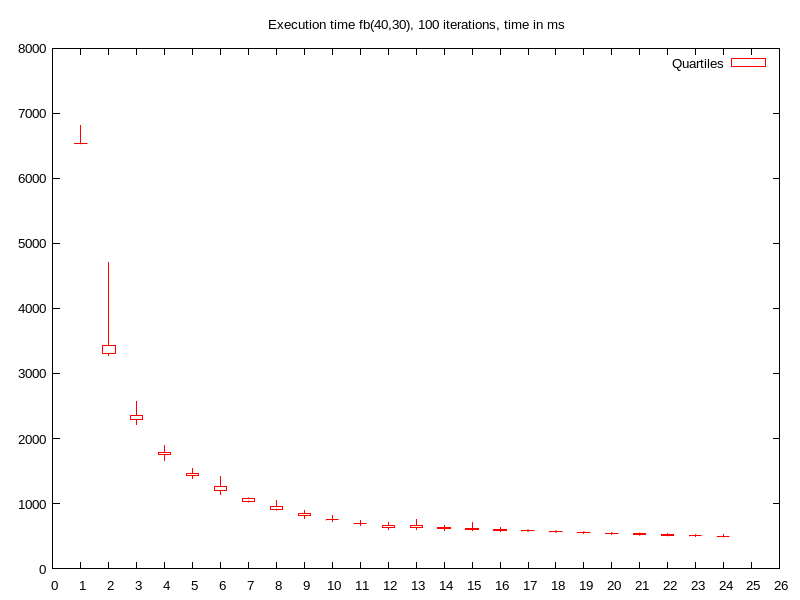
\includegraphics[width=0.6\linewidth]{first.png}

\end{frame}

\begin{frame}{log scale}

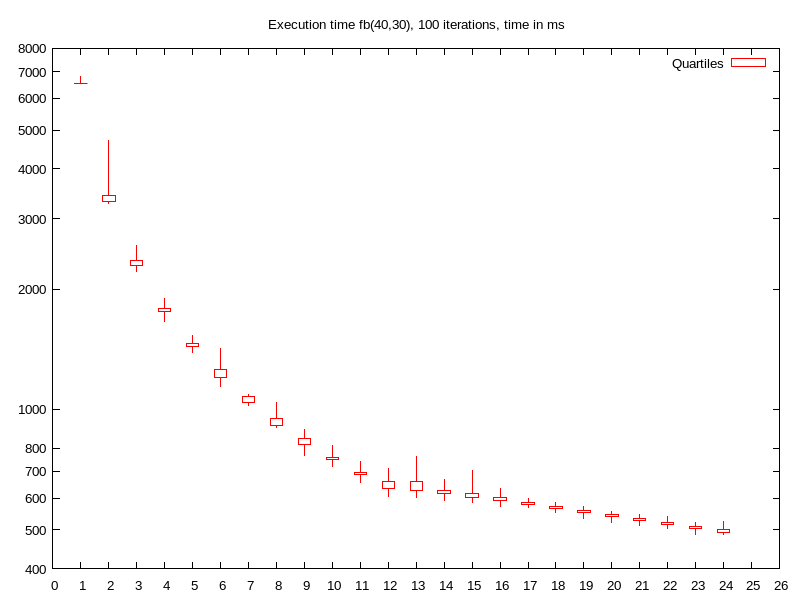
\includegraphics[width=0.6\linewidth]{logy.png}

\end{frame}

\begin{frame}{log-log scale}
 
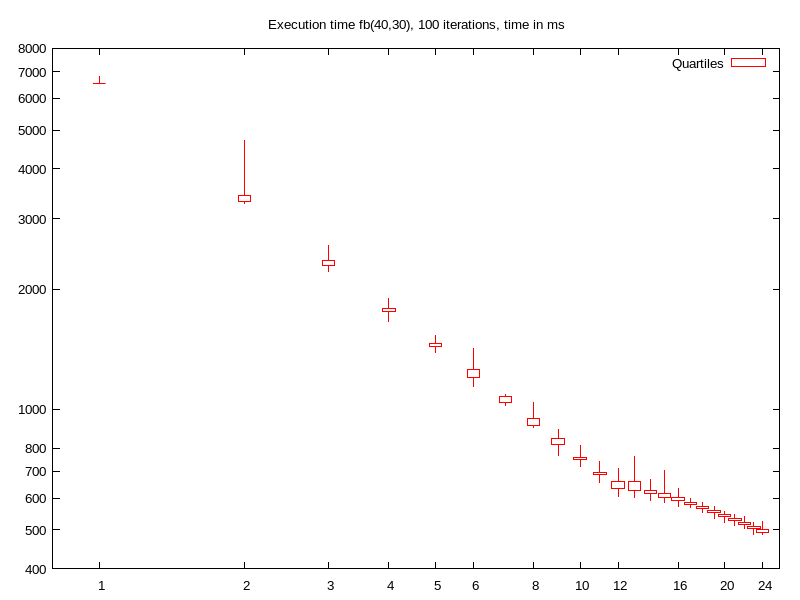
\includegraphics[width=0.6\linewidth]{logxy.png}

\end{frame}

\begin{frame}{as good as it gets}

\begin{itemize}
  \item speed-up 1 - 2 cores : 1.9 %% (/ 6542.0 3415)
  \item speed-up 2 - 4 cores : 1.9 %% (/ 3415.0 1774)
  \item speed-up 4 - 8 cores : 1.9 %% (/ 1774.0 9464)
  \item speed-up 6 - 12 cores : 1.9 %% (/ 1237.0 638)
\pause
  \item speed-up 12 - 24 cores : 1.3 %% (/ 638.0 496)
\end{itemize}

\pause\vspace{20pt}

Calculating Fibonacci in parallel is an example of an ``embarrassingly
easy parallel program''.

\end{frame}

\begin{frame}{Image processing}

Assume that we want to transform an image to a gray scale, and then
reduce the color depth of the image.
\end{frame}


\begin{frame}{question}

  \begin{columns}
    \begin{column}{0.3\linewidth}
      
\includegraphics[width=0.8\linewidth]{hockey.png}
    \end{column}
    \pause
    \begin{column}{0.3\linewidth}
      
\includegraphics[width=0.8\linewidth]{gray.png}
    \end{column}
    \pause
    \begin{column}{0.3\linewidth}
      
\includegraphics[width=0.8\linewidth]{reduced.png}
    \end{column}
\end{columns}

\pause\vspace{20pt}How do we parallelize this?

\end{frame}

\begin{frame}{alternatives}

\begin{itemize}
\pause \item Parallelize the gray transformer and/or the depth transformer, or
\pause \item let the gray transformer feed the color-depth transformer, line by line.
\end{itemize}

\pause\vspace{10pt}{\em A pipe-line: reader - transform - transform - writer}

\end{frame}

\begin{frame}[fragile]{the pipeline}

\begin{verbatim}
  def stream() do
    writer = PPM.writer("reduced.ppm", self())
    reducer = Stream.start(gray_reduce(), writer)     
    grayer = Stream.start(rgb_to_gray(), reducer)     
    PPM.reader("hockey.ppm", grayer)
    receive do
     :done
    end
  end
\end{verbatim}

\end{frame}

\begin{frame}[fragile]{a transformer}
\begin{verbatim}

\end{verbatim}
\end{frame}


\begin{frame}[fragile]{a transformer}
\begin{verbatim}

\end{verbatim}
\end{frame}

\begin{frame}[fragile]{benchmark}

\begin{columns}
 \begin{column}{0.5\linewidth}
\begin{verbatim}
> Test.batch().
reading in  118 ms 
gray in      66 ms 
reduce in    66 ms 
writing in   96 ms 

total in    349 ms
\end{verbatim}
 \end{column}
\pause
 \begin{column}{0.5\linewidth}
\begin{verbatim}
> Test.stream()

 total in 260 ms 
\end{verbatim}
 \end{column}
\end{columns}

\pause\vspace{10pt}
{\em This is using only one scheduler.}

\end{frame}

\begin{frame}[fragile]{benchmark}

\begin{verbatim}
> Test.stream().
reading turning gray, reducing and writing in 260 ms 
\end{verbatim}
\pause
\begin{verbatim}
> erlang:system_flag(schedulers_online, 2). 
1
\end{verbatim}
\pause
\begin{verbatim}
> Test.stream().
reading turning gray, reducing and writing in 161 ms 
\end{verbatim}

\end{frame}

\begin{frame}{a sequence of task}

  Assume we have a sequence of independent task (for example images
  that should processes) how do we parallelize the execution?

\pause\vspace{10pt}
\begin{itemize}
\pause\item pipe-line, each task passes a sequence of processes 
\pause\item task parallel, each task is executed in a separate process
\end{itemize}

\pause\vspace{20pt}{\em Pros and cons?}

\end{frame}

\begin{frame}{stream parallelism}

  Assume we have a flow of events (a twitter feed) and collect
  statistics of the most frequent word during a minute, these words
  are then forwarded to a counter etc.

\pause\vspace{10pt}

  Create a network of processes, each process receives events,
  processes them and forwards them to other processes.

\pause\vspace{20pt}{\em Apache Storm.}


\end{frame}

\begin{frame}{Summary}


\begin{itemize}
\pause\item parallelism vs concurrency
\pause\item concurrency as a tool for parallelism 
\pause\item embarrassing easy parallelism is often easy
\pause\item pipe-line parallelism 
\pause\item task parallelism 
\pause\item stream parallelism
\end{itemize}

\end{frame}

\end{document}
